Pytorch was an easy very intuitive playground to test and experiment with different models, 
optimizers, activation functions and normalization values. The resulting training time and 
accuracy were satisfactory. Here is a table including results from the different combinations
tested:
\begin{table}[H]
    \centering
    \begin{tabular}{|c|c|c|c|c|c|c|}
        \hline
        \textbf{Model} & \textbf{Optimizer} & \textbf{Activation} & \textbf{Norm} & 
        \textbf{Epochs} & \textbf{Accuracy} & \textbf{Time} \\
        \hline
        MLP & Adam & ReLU & Default & 50 & 62.46 & 8.85 \\
        CNN & Adam & ReLU & Default & 50 & 91.58 & 8.63 \\
        CNN & SGD & ReLU & Default & 50 & 91.45 & 8.64 \\
        CNN & Adam & Tanh & Default & 50 & 84.85 & 8.74 \\
        CNN & Adam & ReLU & Standard & 50 & 90.98 & 8.72 \\
        CNN & Adam & ReLU & Zero-cent & 50 & 91.24 & 8.73 \\
        \hline
    \end{tabular}
    \vspace{0.5cm}
    \caption{Different Model Configurations}
\end{table}

Judging from the table, which has taken the console output from the different neural network
configurations and collected it into a single, convenient place, we derive the following 
conclusions:
\begin{itemize}
    \item The training time for all models is very similar.
    \item The CNN model outperforms the MLP model in terms of accuracy.
    \item The Adam and the SGD optimizers are give almost identical results.
    \item The ReLU activation function is the better choice when compared to Tanh.
    \item The default normalization values are basically no different than any of
    the other we tried.
    \item The CNN model with the ReLU activation function and the Adam optimizer
    achieved the highest accuracy of 91.58\%.
\end{itemize}

When it comes to how quickly the models were able to reach high accuracy, the CNN variations
tend to grow faster and peak higher in our particular models. At 10 epoch the CNN model is 
already at 80\% accuracy while the MLP model is still at approximately 55\%. Additionally,
on the CNN model, the test and training accuracy graphs are very close to one another until
the final epochs where the test results fall slightly behind due to over-fitting. The MLP model
on the other hand displays a constant gap between the test and training accuracy graphs where 
the test accuracy graph has a constant 5-10\% lead when compared to the training accuracy graph.
As it seems this is due to the fact that the MLP model hasn't reached its final accuracy yet. 
Here I include the final MLP graph:
\begin{figure}[H]
    \centering
    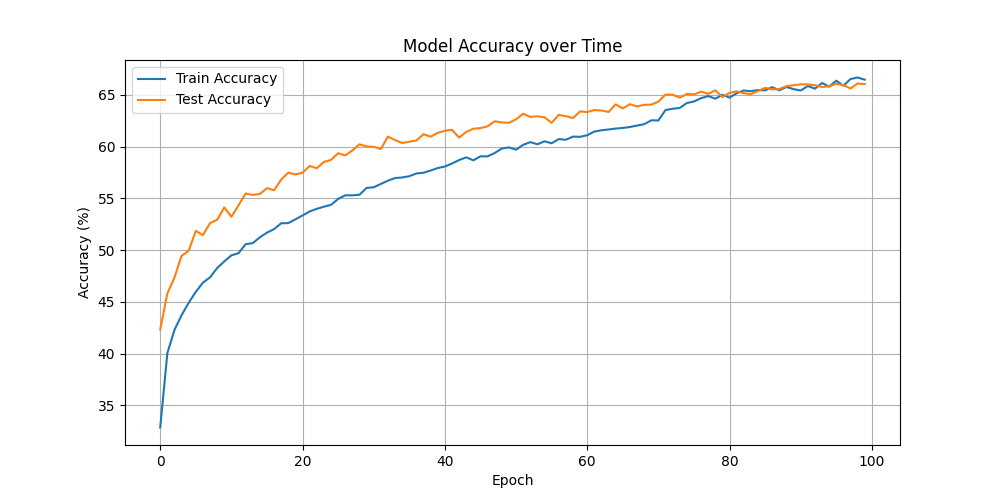
\includegraphics[width=0.5\textwidth]{media/mlp_final_state.png}
    \caption{MLP Final State}
\end{figure}
After around 100 epochs the test accuracy graph converges to the training accuracy graph and the
model reaches its final accuracy of around 67\%. There we can finally see some over-fitting but it
is negligible.

